\section{Introduction}
\label{sec:intro}
From early frame-driven dialog system GUS~\cite{bobrow1977gus} to
virtual assistants~(Alexa, Siri, and Google Assistant \etal),
frame-based dialog state tracking has long been studied to meet
various challenges. In particular, how to support an ever-increasing
number of services and APIs spanning multiple domains has been a focal
point in recent years, evidenced by multi-domain dialog
modeling~\cite{budzianowski2018multiwoz,byrne2019taskmaster,
  shah-etal-2018-bootstrapping} and transferable dialog state tracking
to unseen intent/slots~\cite{mrkvsic2017neural,
  wu2019transferable, hosseini2020simple}.
\begin{figure}[!ht]
\centering
  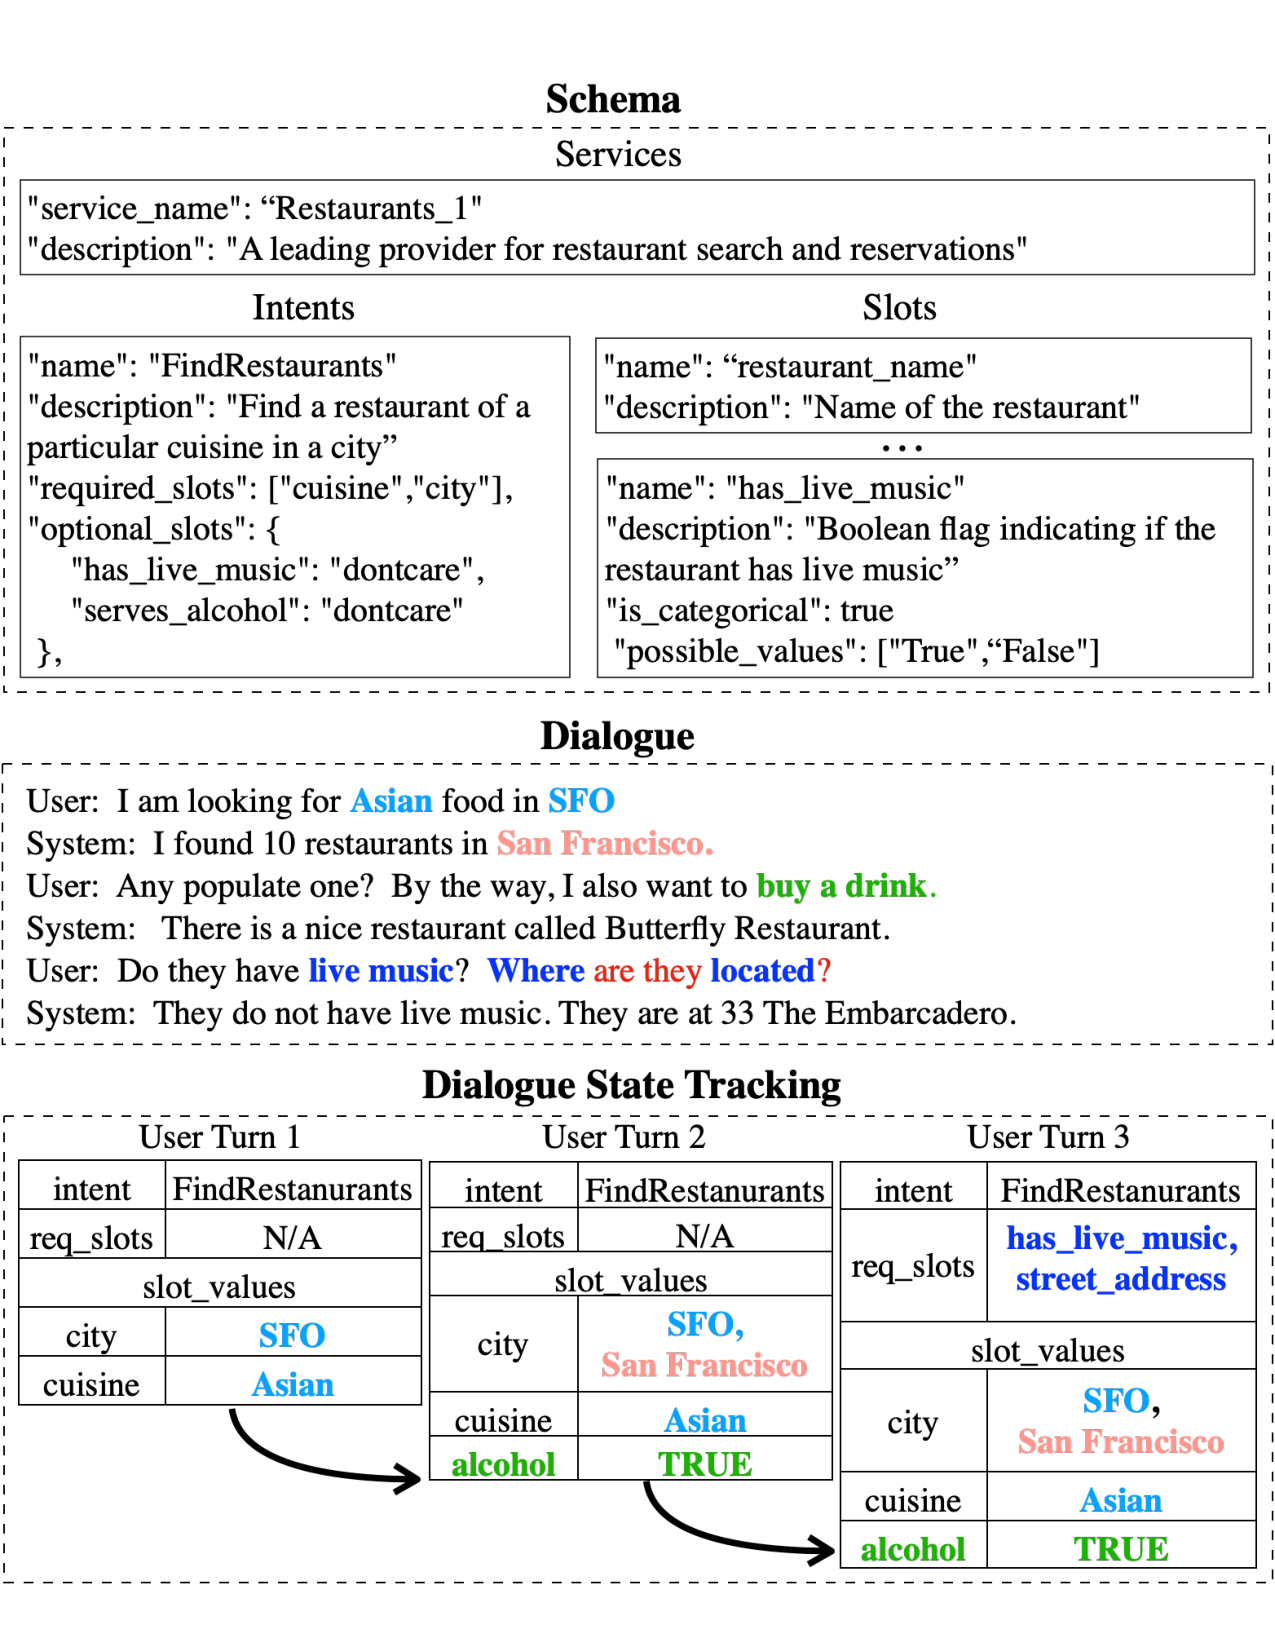
\includegraphics[width=0.47\textwidth]{schema-dst.pdf}
  \caption{\label{fig:schema-dst} An example dialog from Restaurant\_1 service, along with its service/intent/slot descriptions and dialog state representation.}
\end{figure}

Recently, \citet{rastogi2019towards} proposed a new paradigm called
schema-guided dialog for transferable dialog state tracking by using
natural language description to define a dynamic set of service
schemata. As shown in Figure \ref{fig:schema-dst}, the primary
motivation is that these descriptions can offer effective knowledge
sharing across different services, e.g., connecting semantically
similar concepts across heterogeneous APIs, thus allowing a unified
model to handle unseen services and APIs. With the publicly available
schema-guided dialog dataset~(\sgdst~henceforward) as a
testbed, they organized a state tracking shared task composed of four subtasks:
intent classfication~(\IC), requested slot identification~(\RSI),
categorical slot labeling~(\CSL), and noncategorical slot
labeling~(\NSL)~\cite{rastogi2020schema}. Many participants achieved
promising performance by exploiting the schema description for dialog
modeling, especially on unseen services.

Despite the novel approach and promising results, current
schema-guided dialog state tracking task only evaluates on a single
dataset with limited variation in schema definition. It is unknown how
this paradigm generalizes to other datasets and other different styles
of descriptions. In this paper, we focus our investigation on the
study of three aspects in schema-guided dialog state tracking:
\begin{inparaenum}[(1)]
\item schema encoding model architectures
\item supplementary training on intermediate tasks
\item various styles for schema description.
\end{inparaenum}
To make a more general discussion on
the schema-guided dialog state tracking, we perform extensive
empirical studies on both \sgdst~and~\multiwoz~datasets. In summary,
our contributions include:
\begin{itemize}
\item A comparative study
  on schema encoding architectures, suggesting a partial-attention
  encoder for good balance between inference speed and accuracy.
\item An experimental study of supplementary training on
  schema-guided dialog state tracking, via intermediate tasks
  including natural language inference and question answering.
\item An in-depth analysis of different schema description styles on a new
  suite of benchmarking datasets with
  variations in schema description for both \sgdst~and~\multiwoz.
\end{itemize}
%%% Local Variables:
%%% mode: latex
%%% TeX-master: "main"
%%% End:
